\section{Physarum Polycephalum}
\label{section:background_physarum}

The organism being a subject for this work is \textit{Physarum Polycephalum} also called the many-headed slime mould. It is a member of the \textit{Physaridae} family of slime moulds, in order of \textit{Physarales}, class \textit{Myxogastria}, phylum \textit{Myxomycete}, supergroup \textit{Amoebozoa} in \textit{Protista} kingdom. While current position in taxology is well defined, presented characteristics should justify why scientists used to have problems with classification of the Physarum \cite{stephenson1994myxomycetes}.

In order to make the thesis readable, terms \textit{Physarum Polycephalum}, \textit{Physarum} or \textit{the slime mould} will be used interchangeably as the subject is unambiguously defined. As none of the authors have a background in biology, concepts are presented from a computer scientist's perspective in minimal, yet exhaustive, form.


\subsection{Biological characteristics}

\textit{Physarum Polycephalum} is a very peculiar organism. Even being a \textit{Protista} it can be observed with a naked eye --- it is a one amongst biggest living unicellular organisms \cite{stephenson1994myxomycetes}. 

In its natural habitat, under cool, dark and humid conditions the slime mould exists in form of a yellow semistructurised blob (as seen in figure \ref{figure:bp_habitat}). Its occurrence is fairly common around the globe, however species \textit{Physarum Polycephalum} does not occur naturally in Poland \cite{narkiewicz2013grzyby}. It feeds on bacteria, fungi and other sources of basic nutrients (such as aminoacids and carbohydrates).

In laboratory conditions, \textit{Physarum} is stored on Petri dishes filled with non-nutritious agar (figure \ref{figure:bp_petri}). The agar base provides humid environment required for supporting plasmodial stage of the slime mould. A sterile oatmeal or even soft porridge is used as controlled source of nutrients. Complete description of storage and observation protocol, among other information, is provided in Appendix \ref{chapter:protocol}.

\begin{figure}
  \centering
  \begin{subfigure}{0.45\textwidth}
    \centering
    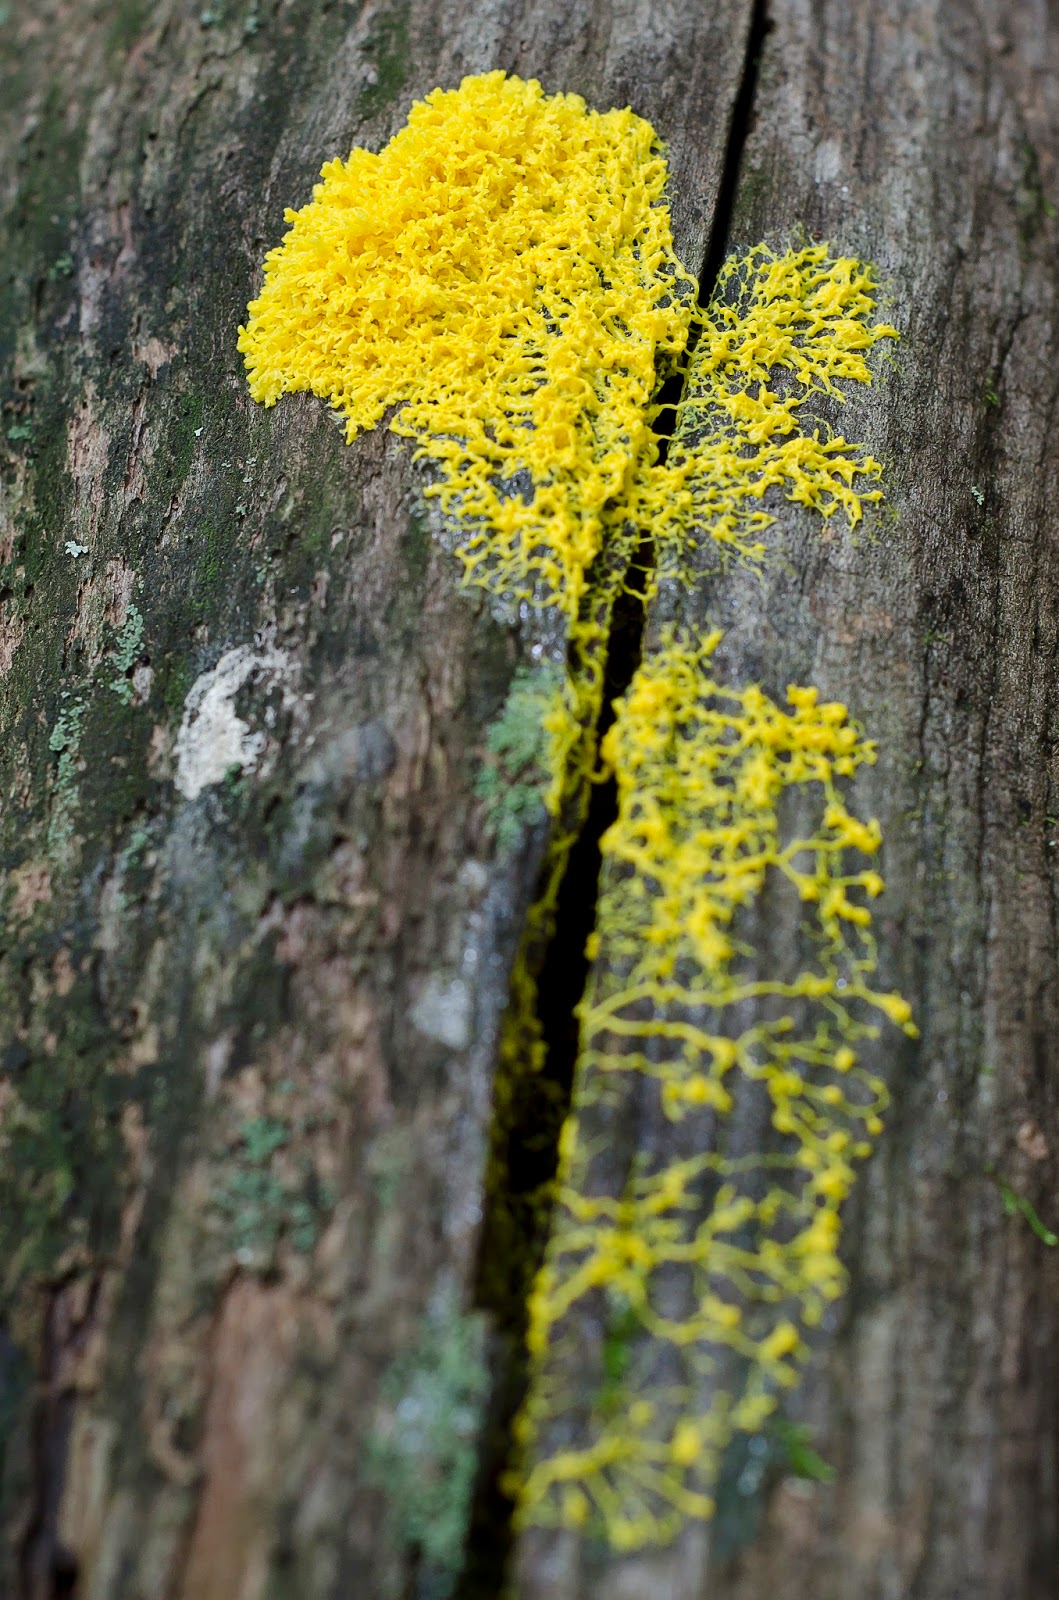
\includegraphics[width=0.9\textwidth]{background/physarum/habitat.jpg}
    \caption{Natural habitat \cite{TODO}}
    \label{figure:bp_habitat}
  \end{subfigure}
  \begin{subfigure}{0.45\textwidth}
    \centering
    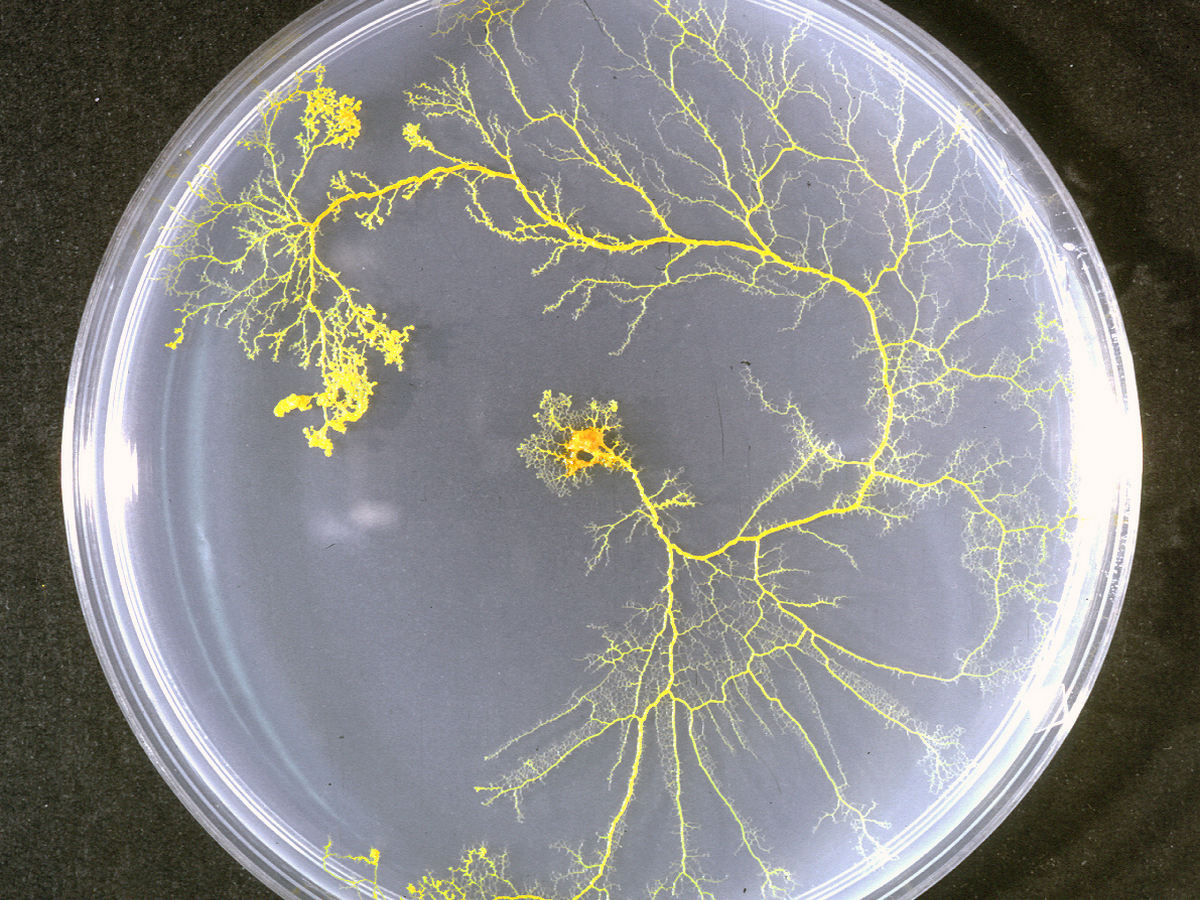
\includegraphics[width=0.9\textwidth]{background/physarum/petri.jpg}
    \caption{Petri dish}
    \label{figure:bp_petri}
  \end{subfigure}
  \caption{\textit{Physarum Polycephalum} in plasmodial stage}
\end{figure}

\begin{figure}
  \centering
  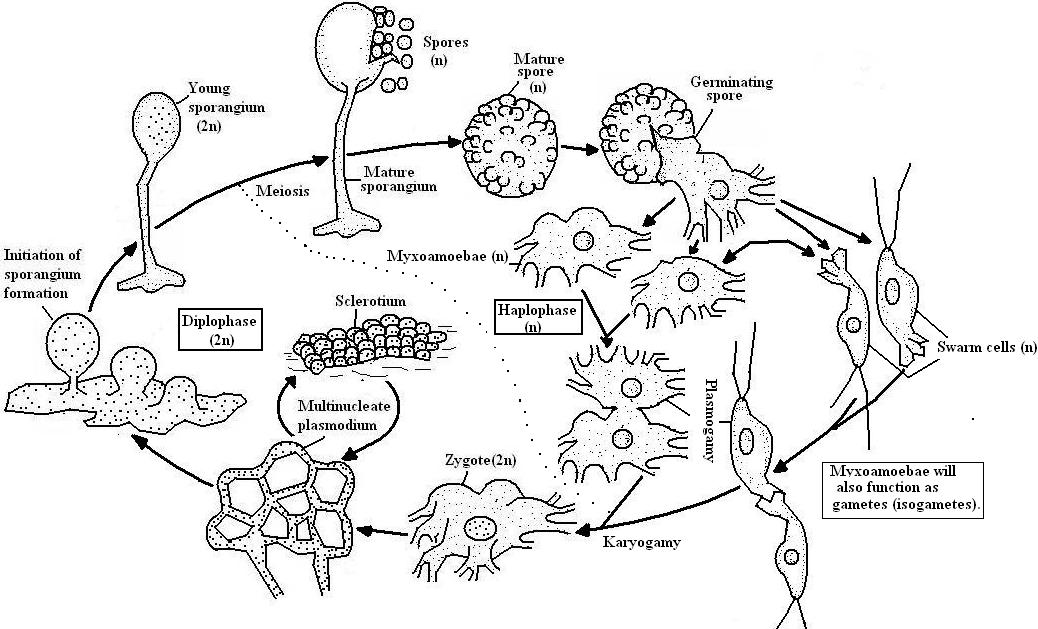
\includegraphics[width=0.94\textwidth]{background/physarum/lifecycle.png}
  \caption{Life cycle of \textit{Physarum Polycephalum} (image source: Carolina Biological Supply)}
  \label{figure:bp_lifecycle}
\end{figure}

As representant of \textit{Myxomycete}, a life cycle of the slime mould is very complex including haploid and diploid phases (as seen in figure \ref{figure:bp_lifecycle}). Such cycle is a result of an evolutionary adaptation. Formation of sporangium occurs as a result of worsening conditions (such as inadequate temperature, humidity or acidity). Sporangium releases spores, which can germinate into ameboid swarm cell. Such cell can enclose itself into a cyst to protect the cells, until environmental conditions improve. When conditions are favourable amoeboid cell turns into flagellated swarm cell. Swarm cells can merge, fuse their nuclei and start mitotic process resulting in forming a plasmodium \cite{jones2015pattern}.

For purposes of unconventional computing applications, \textit{Physarum} is preferred in its plasmodial stage. However, during research transformations into other states are inevitable and must be dealt with. In case of drying or enforced starvation sclerotium is formed --- in this dormant phase \textit{Physarum Polycephalum} can survive for many years until dampness and nutrients are provided again.

Plasmodium forms protoplasmic tubes (also called pseudopodia) accordingly to food availability. Such tubes are used for discovery and transportation of nutrients. The tubes are built in similar way to animal muscles. The ectoplasm contains actin and myosin complexes, which are organised into regular structures forming tubes. Such actomyosin complexes generate contractile motion resulting in streaming of protoplasm. Furthermore, synchronised oscillations of protoplasm stream's direction can observed. Nutrients are transported in one direction, after 1-2~minutes the direction is reversed. Period of this oscillation depends on environment quality and accessibility to food \cite{wohlfarth1979oscillatory} --- higher frequency oscillations are generated where nutrients available and no harmful environment exist, low frequency oscillations are caused by lack of food or as a result of unfavourable conditions. 

The plasmodium can grow around 10~mm per hour when actively exploring environment \cite{coggin1996dynamic}. While moving, plasmodium leaves polysaccharide traces (informally called slime, hence the name slime mould). Network of the protoplasmic tubes adapts, forming efficient ways of transporting nutrients, depending on their amount and quality \cite{nakagaki2004obtaining}. Exploiting this behaviour is a fundamental principle for building physarum machines.


\subsection{Related works}

Since early 1960s \textit{Physarum Polycephalum} has been a subject to many biological and microbiological studies \cite{guttes1964mitotic,daniel1962method}, however it is late 70s when its computational-like behaviours have been observed \cite{wohlfarth1979oscillatory}.

% TODO artists
Research towards computational applications of the \textit{Physarum} truly started in 1990s. Nowadays, there exist two prominent research centres focusing on the slime mould --- one based in United Kingdom (Andrew Adamatzky\footnote{~\url{http://uncomp.uwe.ac.uk/adamatzky/}}, Jeff Jones\footnote{~\url{http://uncomp.uwe.ac.uk/jeff/}} from University of West England, Bristol), other one in Japan (Toshiyuki Nakagaki\footnote{~\url{http://www.cris.hokudai.ac.jp/cris/en/research/ob/ob\_innovative/nakagaki.html}}, Hokkaido University, Sapporo). Some of their works excited us about slime mould capabilities and inspired to write this thesis \cite{nakagaki2000intelligence,adamatzky2010physarum,jones2015pattern,adamatzky2007physarum}. Experiments presented here focus on different aspects of \textit{Physarums} behaviour. Analysing and understanding them gives impression of emerging computational power of such simple organism as a slime mould.


\subsubsection{Maze-solving capabilities}

Maze-solving or more constricted problem of finding, preferably shortest, paths is very common in practice. It has many applications and many possible algorithms are already available. Algorithms such as breadth-first search or more complex $A*$ are commonly used for solving mazes \cite{zelkowitz1979principles}, however Toshiyuki Nakagaki et al. proposed usage of slime moulds' natural capabilities as unconventional solution to this problem \cite{nakagaki2000intelligence}.

In order to use \textit{Physarum} to solve a labyrinth, a maze must be represented as a physical object. Such maze is modelled on a Petri dish where floor is made of non-nutrient agar and walls are made of thin plastic film (the maze used in the experiment is presented on figure \ref{figure:bp_maze_initial}). As the slime mould strictly prefers humid environment of the agar it will not pass arid walls made of plastic film. 

\begin{figure}
  \centering
  \begin{subfigure}{0.45\textwidth}
    \centering
    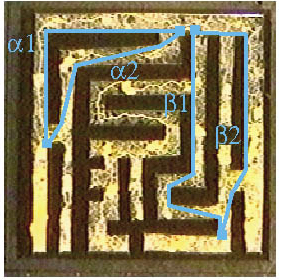
\includegraphics[width=0.9\textwidth]{background/physarum/maze1.jpg}
    \caption{Plasmodium initially filling maze}
    \label{figure:bp_maze_initial}
  \end{subfigure}
  \begin{subfigure}{0.45\textwidth}
    \centering
    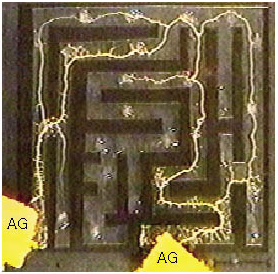
\includegraphics[width=0.9\textwidth]{background/physarum/maze2.jpg}
    \caption{Intermediate state}
    \label{figure:bp_maze_intermediate}
  \end{subfigure}
  \begin{subfigure}{0.45\textwidth}
    \centering
    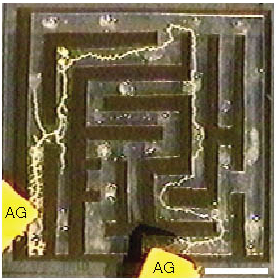
\includegraphics[width=0.9\textwidth]{background/physarum/maze3.jpg}
    \caption{Final route}
    \label{figure:bp_maze_final}
  \end{subfigure}
  \caption{\textit{Physarum} in various states of the maze experiment \cite{nakagaki2000intelligence}}
\end{figure}

There are four possible routes available $\{(\alpha_1,\beta_1), (\alpha_1,\beta_2), (\alpha_2,\beta_1), (\alpha_2,\beta_2)\}$ between entry point $A$ and exit point $B$. Oatmeal-agar-based source of nutrients is planted in both entry and exit points, while large enough plasmodium is placed over whole floor of the maze. As time passes it can be observed that plasmodium retracts its body from labyrinth's dead-ends, leaving traces of slime where it previously has been placed (figure \ref{figure:bp_maze_intermediate}). 

As a result the slime mould rests only on direct paths connecting the entry with an exit point (figure \ref{figure:bp_maze_final}). Furthermore, it has been observed that \textit{Physarum Polycephalum} usually prefers shortest $(\alpha_2,\beta_1)$ path as it prefers most efficient way for transferring nutrients. While obtained results are satisfactory, it must be noted that whole process takes about 4~hours. 


\subsubsection{Spatial memory}

Memory is usually associated with neurological functions of brain, however it can be externalised in multiple ways, in example as pheromone trails of ants \cite{carroll1973ecology} or even notes-writing as humans do \cite{fisher1973effect}. Team of researchers from University of Sydney, demonstrated that \textit{Physarum Polycephalum} uses its slime as a form of spatial externalised memory \cite{reid2012slime}.

A common problem testing autonomous navigational skills in robotics is U-shaped trap problem \cite{chatterjee2001use}. Efficient solution of the issue requires some kind of spatial memory or other navigational aids \cite{balch1993avoiding}, therefore it was a good candidate for a test of slime mould's memorising capabilities. The U-maze problem requires an agent (a robot or as in this example the slime mould) to navigate itself from starting position to the goal, where goal is hidden beside the U-shaped trap (figure \ref{figure:bp_trap_model}). The agent has to use some kind of environment map or use reactive guidance to bypass the trap (figure \ref{figure:bp_trap_model_success}), otherwise, most probably it will be stuck inside the trap (figure \ref{figure:bp_trap_model_failure}).

\begin{figure}
  \centering
  \begin{subfigure}{0.33\textwidth}
    \centering
    \includegraphics[width=0.9\textwidth]{background/physarum/trap_initial.eps}
    \caption{Initial setup}
    \label{figure:bp_trap_model}
  \end{subfigure}
  \begin{subfigure}{0.37\textwidth}
    \centering
    \includegraphics[width=0.9\textwidth]{background/physarum/trap_success.eps}
    \caption{Example successful route to goal}
    \label{figure:bp_trap_model_success}
  \end{subfigure}
  \begin{subfigure}{0.37\textwidth}
    \centering
    \includegraphics[width=0.9\textwidth]{background/physarum/trap_failure.eps}
    \caption{Typical failure}
    \label{figure:bp_trap_model_failure}
  \end{subfigure}
  \caption{U-trap test with possible outcomes}
\end{figure}

The experiment conducted by Reid, Latty, Dussutour and Beekman \cite{reid2012slime} used \textit{Physarum Polycephalum} as an agent in non-nutrient agar environment, where the trap was made out of acetate and the goal was highly nutritious glucose. The agar base allows diffusion of glucose particles, creating nutrients gradient towards the goal.

Initial experiments indicated that \textit{Physarum} moves in direction where its slime is not present, however if no such direction exists (there is the slime all around plasmodium) it moves in random direction or all over the substrate. Therefore a slime mould has a choice to explore unexplored, however it is not an ultimate one, as it always can maneuver in previously visited areas. 

\begin{figure}
  \centering
  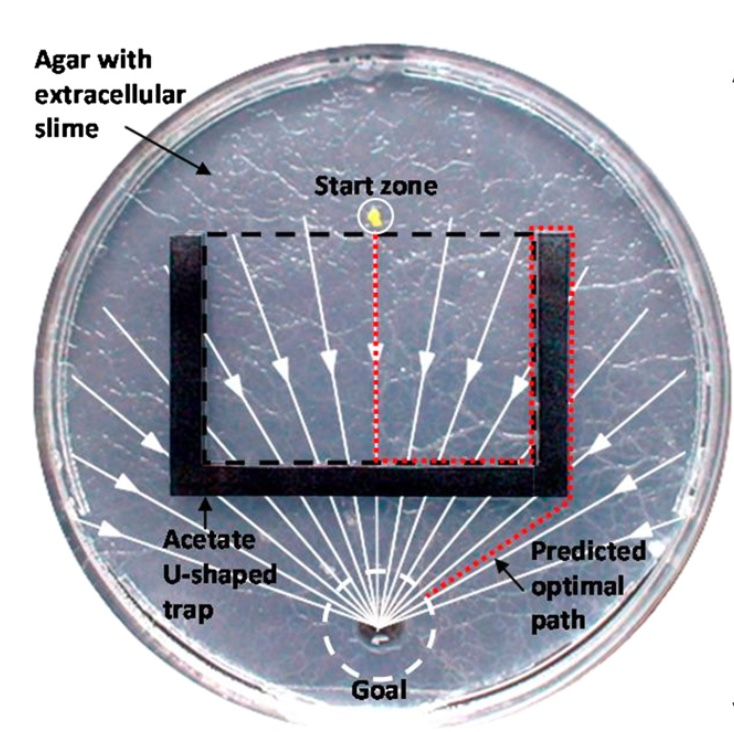
\includegraphics[width=0.74\textwidth]{background/physarum/trap_experiment.jpg}
  \caption{\textit{Physarum Polycephalum} in U-trap experiment on a slime covered substrate \cite{reid2012slime}}
  \label{figure:bp_trap_experiment}
\end{figure}

As the slime is stable, nonliving substance mostly made of galactose polymers it can be easily handled, collected and replanted \cite{mccormick1970isolation}. Two varieties of the experiment has been designed --- in a first one, previously collected slime is placed all over the substrate (figure \ref{figure:bp_trap_experiment}), where in a second one the substrate is just a clean agar. The first environment constrains \textit{Physarum} not to rely on slime for navigation (as provided slime acts as noise), unlike the second one, in which \textit{Physarum} can use the slime freely for its navigation.

Experiments have shown that \textit{Physarum} placed on a substrate already coated with the slime cannot easily escape out of the U-trap --- it spends there a long time until it leaves the trap. Furthermore, only in 33\% of 24 repeated cases plasmodium reaches the goal. However, when plasmodium is put on a clean agar substrate, an ability to use its slime as navigational aid results in reaching the goal in 96\% of cases. Both, travelled distance and time to reach the goal, were much shorter when the organism were able to use the slime. These findings prove that \textit{Physarum Polycephalum} can sense its extra-cellular slime and uses its existence as form of externalised spatial memory for recognition of previously explored areas.


\subsubsection{Adaptive network design}

Networks are used in a variety fields of engineering --- from civil roads, water pipelines, railway systems to energy grids, not to mention the Internet. Design of a practical robust network usually implies a balance between efficiency, cost and fault tolerance. Increasing robustness involves creation of redundant connections between some of the nodes. This might seem not to be profitable, however it allows network to gracefully degrade and still maintain some of its throughput. Japanese team of scientists showed that \textit{Physarum Polycephalum} can be used to design networks on a par with human or algorithmic designs \cite{tero2010rules}.

% TODO remove letters from pictures
\begin{figure}
  \centering
  \begin{subfigure}{0.33\textwidth}
    \centering
    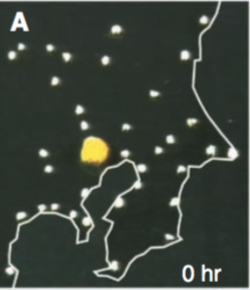
\includegraphics[width=0.9\textwidth]{background/physarum/network_initial.jpg}
    \caption{Initial placement}
    \label{figure:bp_network_initial}
  \end{subfigure}
  \begin{subfigure}{0.33\textwidth}
    \centering
    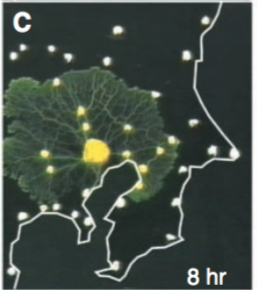
\includegraphics[width=0.9\textwidth]{background/physarum/network_intermediate_a.jpg}
    \caption{State in $t=8h$}
    \label{figure:bp_network_intermediate_a}
  \end{subfigure}
  \\
  \begin{subfigure}{0.33\textwidth}
    \centering
    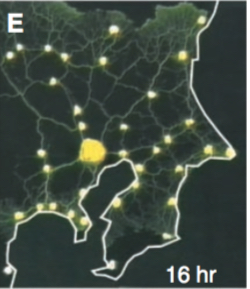
\includegraphics[width=0.9\textwidth]{background/physarum/network_intermediate_b.jpg}
    \caption{State in $t=16h$}
    \label{figure:bp_network_intermediate_b}
  \end{subfigure}
  \begin{subfigure}{0.33\textwidth}
    \centering
    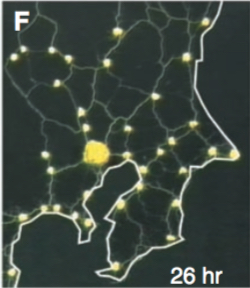
\includegraphics[width=0.9\textwidth]{background/physarum/network_final.jpg}
    \caption{Final plasmodium state}
    \label{figure:bp_network_final}
  \end{subfigure}
  \caption{Example \textit{Physarum Polycephalum} network in railway experiment \cite{tero2010rules}}
\end{figure}

The choice of the slime mould was quite natural: the organism forms a network as it forages and it can be assumed, that trough uncountable years of evolution, its designs has reached an equilibrium between cost, efficiency and robustness. The researchers prepared an experiment based on design of Tokyo-area rail network. On a substrate made of agar thirty~six~food~sources (identical oat meals) have been placed as in topographical positions of the rail stations (figure \ref{figure:bp_network_initial}). A blob of plasmodium has been placed where city of Tokyo would be, after some time, as the slime mould forages, it covered the substrate and connected each food source (figures \ref{figure:bp_network_intermediate_a}, \ref{figure:bp_network_intermediate_b}). Afterwards \textit{Physarum} retracted its body from the empty areas, leaving only interconnected food sources (figure \ref{figure:bp_network_final}). It should be observed, that some junctions have been left where no food is placed --- these are Steiner~points \cite{kou1981fast} enhancing overall efficiency of the network.

The experiment has been replicated 20~times, each time resulting in slightly different design of the final network, however it always resembled a Tokyo rail network designed by civil engineers. In order to even further improve similarity, the substrate has been illuminated where geographical features restrain the rail network. As the slime mould avoids light, such illumination acted as a constraint for the network --- these networks bore even bigger similarities to original plans than networks made without constraints. 

In the end, it was concluded that networks designed by \textit{Physarum Polycephalum} have lower overall cost with similar transport efficiency, however they lack a bit of fault tolerance --- while in only 4\% of faults the real rail network would lead to isolation of any part, in case of networks designed by the slime mould such isolation would occur in 14\% of faults. Still, these results are acceptable as \textit{Physarum}'s network designs have much lower cost. Nonetheless, it should be noted that these networks should not be compared directly --- stops on Tokyo network have not been planned at once, they evolved as the city grew, unlike the task given to \textit{Physarum} which assumed knowledge of stops locations. The processes differs even more, as design of real rail network is usually centralised, however the slime mould acts as self-organised mechanism without central control.


\subsubsection{Slime mould models}

In the same work \cite{tero2010rules} Japanese researchers proposed a mathematical model of \textit{Physarum Polycephalum} used for adaptive network designs based on a flow network. The slime mould has been adapted as initially random lattice, where edges represents the pseudopodia. The flux inside pseudopodia has been accurately defined with Hagen-Poiseuille formula for laminar flow \cite{sutera1993history}. Simulation is conducted in discrete time steps, in each step a random food source node is selected to drive the flow through the network, where another food source is selected to be a sink. Strength of the flow influences conductivity of each tube --- unused tubes gradually disappear, while effective tubes adapt to increase throughput. This model reflects some of the properties of the real slime mould and can be used for design of adaptive network model.

Quite profound work on modelling \textit{Physarum Polycephalum} has been presented by Jeff Jones in his book \cite{jones2015pattern}. He modelled plasmodium in multi-agent fashion as a material made of multiple particles working towards reaction-diffusion process. A single agent represents a particle of plasmodium gel/sol structure --- its movement resembles protoplasmic flow, however when it is immobile, it could be treated as gel matrix. Each agent can sense chemoattractants in two-dimensional substrate using three forward-directed sensors. A single agent can move in oscillatory or non-oscillatory modes, where first one can be used to approximate resistance within plasmodium and the second one represents ideal movement without any external forces. Plasmodium-like behaviour emerges from collection of such randomly placed agents. Furthermore chemoattractants and chemorepellents can be placed on the substrate, stimulating the agents to regroup and move. This model can be tuned to closely resemble real \textit{Physarum Polycephalum} in a variety of environment conditions.

% TODO crop images so they are aligned
\begin{figure}
  \centering
  \begin{subfigure}{0.3\textwidth}
    \centering
    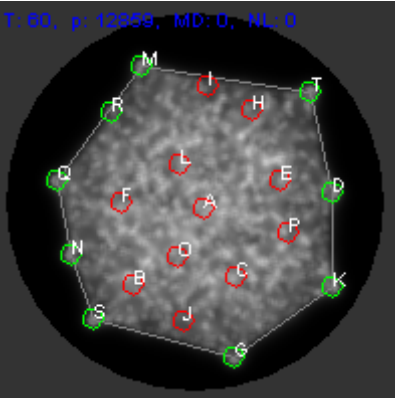
\includegraphics[width=0.9\textwidth]{background/physarum/tsp_initial.png}
    \caption{Initial placement within convex hull}
    \label{figure:bp_tsp_initial}
  \end{subfigure}
  \begin{subfigure}{0.3\textwidth}
    \centering
    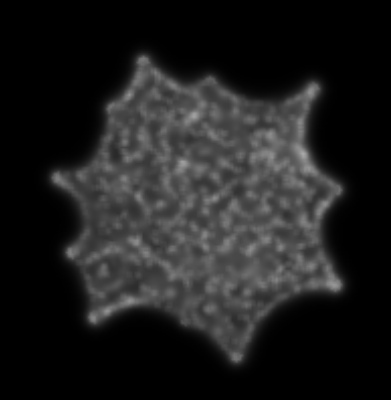
\includegraphics[width=0.9\textwidth]{background/physarum/tsp_intermediate.png}
    \caption{State after removal of some agents}
    \label{figure:bp_tsp_intermediate}
  \end{subfigure}
  \begin{subfigure}{0.3\textwidth}
    \centering
    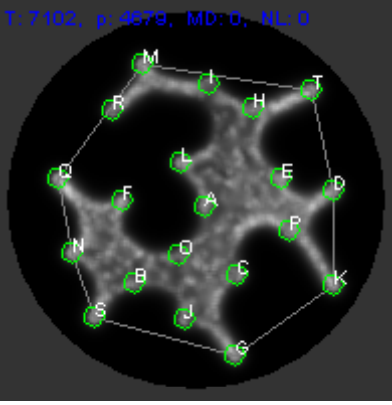
\includegraphics[width=0.9\textwidth]{background/physarum/tsp_final.png}
    \caption{Final state of simulation}
    \label{figure:bp_tsp_final}
  \end{subfigure}
  \caption{Solving TSP using shrinking blob method \cite{jones2014computation}}
\end{figure}

\begin{figure}
  \centering
  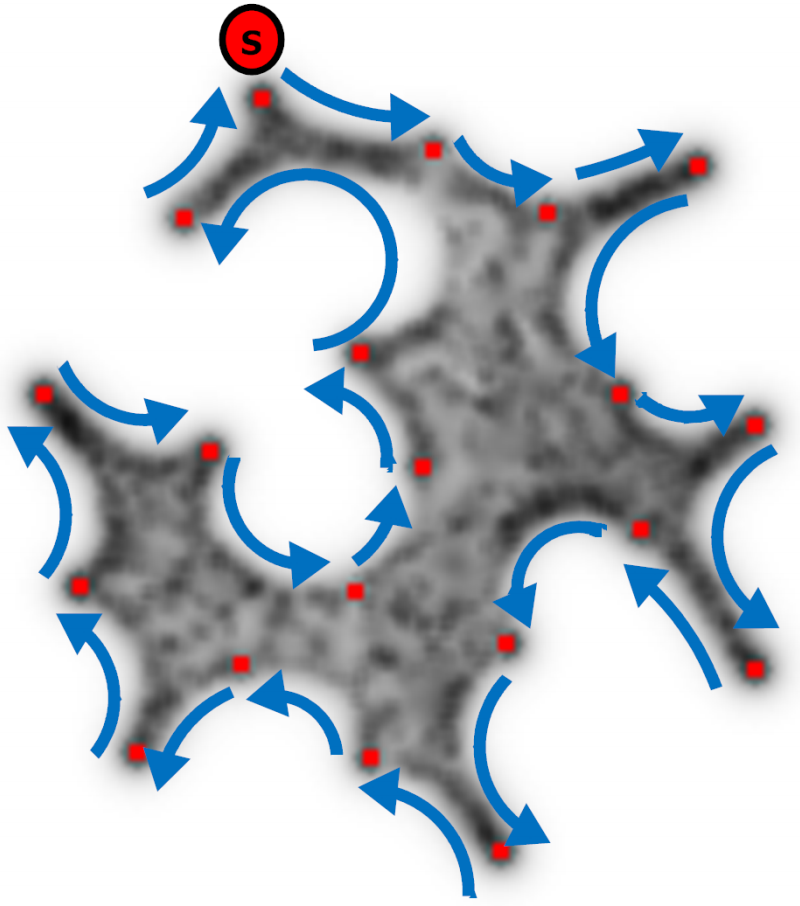
\includegraphics[width=0.3\textwidth]{background/physarum/tsp_readout.png}
  \caption{TSP tour readout method \cite{jones2014computation}}
  \label{figure:bp_tsp_readout}
\end{figure}

Based on this model Jeff Jones and Andy Adamatzky proposed a method of shrinking blob for approximating solution of Travelling Salesman Problem \cite{jones2014computation}. This method requires putting previously described agents inside a convex hull computed on topology of TSP input (figure \ref{figure:bp_tsp_initial}). Initially chemoattractants are placed nearby data points, as simulation goes some agents are removed from the virtual plasmodium, effectively shrinking the blob (figure \ref{figure:bp_tsp_intermediate}). Simulation is stopped when each node is partially uncovered --- a $5 \times 5$ window passes over each node and checks for such condition (figure \ref{figure:bp_tsp_final}). Resulting TSP tour can be read by tracking perimeter of the blob at the end of simulation (figure \ref{figure:bp_tsp_readout}). The authors evaluated this method to be 4.27\% worse than optimal solutions in their dataset.


\subsection{Observations}

We were lucky to be in possession of \textit{Physarum Polycephalum} culture obtained from Carolina Biological Supply. The access to the living organism allowed us to observe its behaviour in variety of conditions. As for computer scientists, who have not previously done any wet lab works, it was a very educational challenge to handle alive slime mould --- detailed methods of handling are presented in Appendix \ref{chapter:protocol}.

Usually we worked with the slime mould on 2\% non-nutrient agar substrate, however two other substrates have been tested. We have placed plasmodium on dampened kitchen towel, as they are easier to manage than agar solution --- no mobility has been affected, however water evaporated quickly and regular moisturising has been required. Furthermore moving colony out of the kitchen towel was more complicated, as it was difficult to cleanly separate the organism from the substrate. An aluminium foil has been tested as substrate too, while it makes the separation easy it was not used for long, as this substrate lacks ability to bound water, which is required for keeping \textit{Physarum Polycephalum} in its plasmodial stage. A standard non-nutrient agar keeps moisture for a long time (up to 10 days until the plasmodium is moved to new substrate) and keeps smooth surface if properly poured into Petri dish, making it quite easy to relocate the colony. Agar gel-like structure prohibits \textit{Physarum} from escapades to the bottom part of Petri dish, unlike porous kitchen towel. 

We used classic oatmeal as primary food for the slime mould. It is composed primarily of starch, some proteins, little fat and trace amount of sugar. We usually used oats as a whole or smaller distinct pieces, but for even bigger precision a sterile porridge paste has been used. Nutrients available in oatmeal made the plasmodium move with 9--10~mm/hr (measured on frontier). We experimented with use of table sugar as nutrient, resulting in 8~mm/hr velocity and decolorisation of the plasmodium. Usage of syrup made of pure glucose made the subject to move relatively fast 12--16~mm/hr, however it was completely decolorised and no networking behaviour was observed. It is possible that glucose has dissolved within an agar substrate changing the slime mould's foraging strategy to the simpler one --- no need to look for food as the substrate became source of nutrients. We also confirmed that valerian drops made from valerian root act as strong chemoattractant for the slime mould \cite{adamatzky2012physarum} --- given choice of oatmeal and oatmeal mixed with valerian drops \textit{Physarum} foraged towards the second one in ten of ten cases. Additionally, when multiple sources of food, varying in their size, were introduced to a slime mould, it always ended up foraging on the largest one. In the end we reaffirmed that oatmeals are preferred source of nutrients for laboratory use. As for water, distilled water was used, however when no access to such pure water was possible a tap water has been used. We observed that tap water slightly decreased \textit{Physarum} mobility to abound 8-9~mm/hr, with no other consequences --- it could be caused by chlorine or fluorine used for tap water disinfection \cite{uden1983chlorinated}.

The culture of \textit{Physarum Polycephalum} has been kept in dark shoebox as these conditions are favourable for growth of plasmodium \cite{adamatzky2010physarum}. When the slime mould has been kept in a window-lit room, plasmodium growth has been massively reduced (none to as little as 4~mm/hr). However we found that infrared light (near-IR LED has been used) made no observable effects on the plasmodium --- one can use infrared light and infrared camera to observe plasmodium as it forages in the dark. We are assuming that infrared light carries little enough energy, so it makes no harm to the organism. When the Petri dish has been partly lit with visible light \textit{Physarum} strongly avoided bright areas --- it stayed at most 5~mm close to the light patch (as some light has been diffused within agar substrate). A green laser (20~mW power, 520~nm wavelength) has been used with similar results, however the area was lit more precisely. 

Pattern of light can be used to create constraints for the plasmodium --- arrangement of LEDs or lasers can be used for precise limits, some even propose usage of gobo lights or projectors for complex patterns \cite{zhu2013amoeba}. Constraints can be also made using physical or chemical methods. We tested table salt and easily obtainable citric acid as potential chemorepellents. A line made of table salt became an obstacle for crawling plasmodium, it never crossed this line, instead the slime mould bypassed around such obstacle. Same effects have been observed with the citric acid crystals, furthermore enclosing the slime mould within a circle made of citric acid effectively reduced its foraging area to within the circle. While chemical repellents are effective, in a longer term they dissolve into agar substrate, contaminating it and making it unsuitable for keeping the subject alive. Physical based obstacles can be solution to this problem. We tested two solutions --- removal of agar substrate and addition of thin plastic sheet. Both methods are exploiting the fact that \textit{Physarum} requires a wet substrate to keep its active plasmodial stage, thus it avoids dry areas. The first method requires cutting out some of the agar resulting in exposing dry area of the Petri dish, where the second one requires cutting pieces of plastic (we used thin yet hard polypropylene foil) and putting them on top of substrate creating dry area. Both methods are de facto effective, however we observed unlikely cases (2 out of 10 experiments) where plasmodium has crossed such physical barrier. This observation can be compared to behaviour of an electrical current, which follows path of least resistance, but if insulator is not thick enough it actually can be bypassed --- indeed, usage of thicker physical barriers makes them more robust. 

Hereafter we can conclude that creating barriers is a tradeoff between side~effects and complexity:
\begin{itemize}
  \item light-based --- have no side effects, but are complex to create,
  \item chemical --- easy to create, but with catastrophic long-term effect,
  \item physical --- moderate to create, but somehow unreliable, occupying large area.
\end{itemize}

% TODO add image
The slime mould fed with oatmeal on an agar substrate forages in network structure. Individual oatmeals are connected by pseudopodia varying in thickness. Width of protoplasmatic tubes is proportional to nutrients transported with the flux between nodes of the plasmodium. The organism created many nodes where no food have been placed, thus optimising paths for the nutrients. Moreover during experiments with various food sources and barriers, regular changes in width of the tubes have been observed as response to the local environment. The pseudopodia thickness changed up to 20\% over time span of 60-170 seconds --- frequency of such oscillation has been greater near positive stimulus (food source), lower frequencies have been observed in tubes closer to chemorepellents (such as salt). This behaviour can be used as a form of communication between \textit{Physarum} and other devices --- a time-lapse imaging can be used to acquire such reaction, further processing with Fourier transform \cite{bracewell1965fourier} could be used for interpretation of positive and negative feedback from the \textit{Physarum Polycephalum}.

Virtually every research available simplifies \textit{Physarum Polycephalum} to a two-dimensional being --- every experiment is conducted on flat Petri dish, pictures are two dimensional etc. By accident we discovered that the slime mould can make three dimensional structures. When it was kept in a Petri dish with lid closed, with plenty of nutrients in form of oatmeal and well humidified air, plasmodium crawled to the lid, later on dripping from the lid to the bottom of the dish. In the end structures resembling stalagnates have been formed, making the slime mould a three dimensional creature. While some may find this observation somehow useful in designing their experiments, it should be noted that observation of such structures and feeding the organism is complicated as once made they prevent Petri dish from opening. 

